\documentclass{ximera}  


\input{../preamble.tex}



 
\title{Electrostatic Field} 
\author{Milica Markovic} 
\outcome{Explain definition of electric field. Derive and calculate electric field due to several point charges using vector algebra. }
\begin{document}  
\begin{abstract}  

\end{abstract}  
\maketitle    




\subsection{More about the Electrical force and field}

We talked about the Electric Force in the previous section. To find the force on one charge, we had to know the position of all charges and what is their charge.  To introduce Electric Field, we'll call charge $q_1$ the source of the force and charge $q_2$ the charge that feels the force. Charge one produces the force, and charge two feels the force. 

By introducing the concept of the field, we can separate the cause of the field and the effect that the field has on other charges. We can find a field due to a charge or charge distribution, and once we know this field, we don't have to keep track of the source charge. We can just find the field's effect on other charges or charge distributions.


 In the Equation \ref{forceField1} $q_1$ and $q_2$ are charges, r is the distance between the two charges, and $\hat{r}$ is the unit vector directed  from charge one to charge two. The electric field of a source charge $q_1$ is defined as the force that a charge $q_1$ would impress on a positive charge $q_2$, divided by the amount of charge $q_2$, as shown in Equation \ref{definitionOfField}. One thing to remember is that in the definition of the electric field, we always assume that the charge $q_2$ is positive! This way, we remove the ambiguity of the field direction. The direction of the electric field at a point P from charge $q_1$ is always in the direction of the force that would act on a positive charge $q_2$ placed at that point, as shown in Figure \ref{UnitCh1}.


\begin{eqnarray}
\vec{F_2}=\frac{q_1 q_2}{4 \pi \epsilon r^2 } \hat{r} \label{forceField1}\\
\vec{E} = \frac{\vec{F_2}}{q_2} \label{definitionOfField} \\
\vec{E} =  \frac{q_1}{4 \pi \epsilon_0 r^2} \hat{r} \label{electricfield}
\end{eqnarray} 

If you carefully look at the Equation \ref{electricfield}, you see that the electric field depends only on the source charge $q_1$. 

\begin{figure}[htbp]
\begin{center}
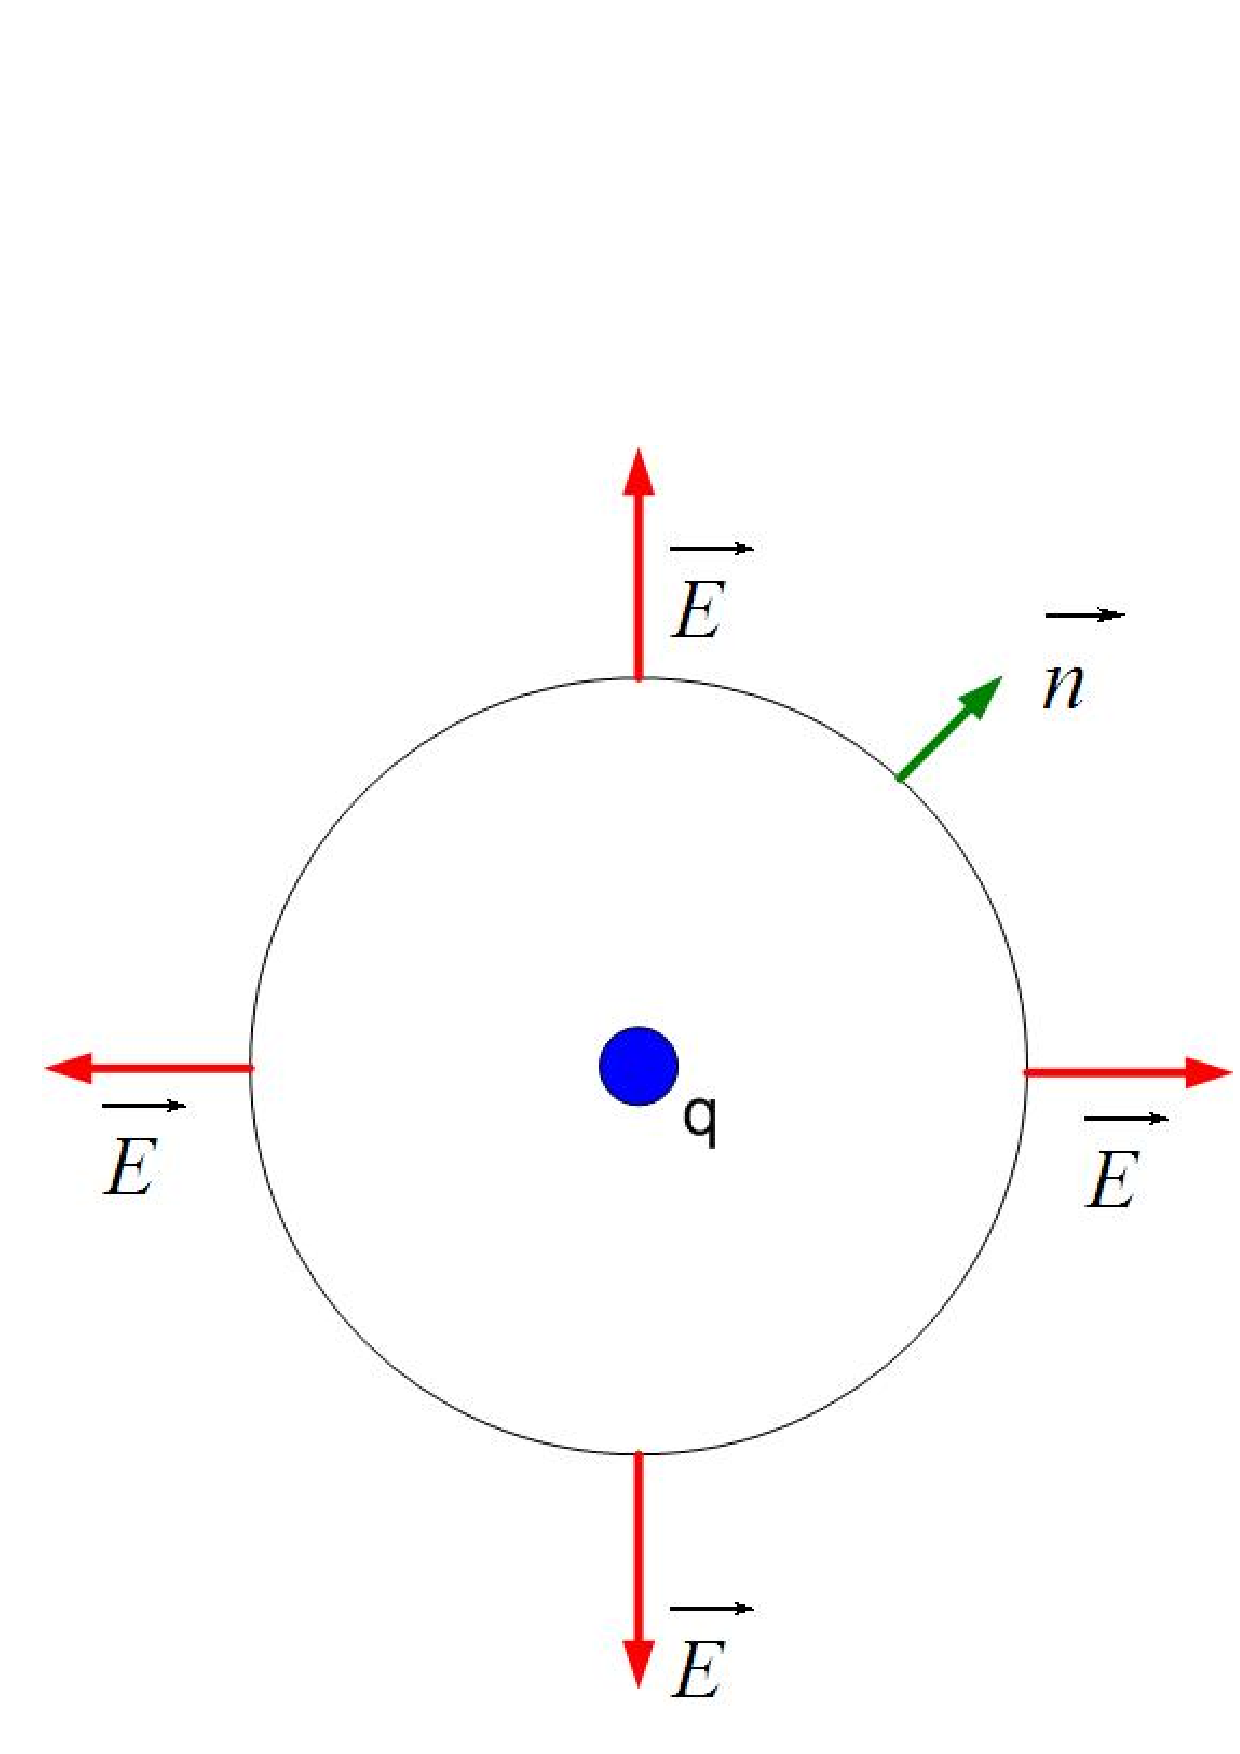
\includegraphics[scale=0.5]{../jpg/unitchargefield.jpg}
\end{center}
\caption{Electric field due to a unit charge q.}
\label{UnitCh1}
\end{figure}

If the electric charge is in a medium other than air, the electric field becomes


\begin{eqnarray}
\vec{E}=\frac{q_1 }{4 \pi \epsilon_0 \epsilon_r r^2} \hat{R_{12}} \\
\epsilon = \epsilon_0 \epsilon_r
\end{eqnarray}\label{Coulombslaw3}

We added a unitless quantity, $\epsilon_r$, called the relative dielectric constant, or relative permittivity, of a material. $\epsilon_r$ values for different materials can be found online. For example, you can see its values for different materials here  \url{https://en.wikipedia.org/wiki/Relative_permittivity.}




\begin{problem}
   Find the electric field at a center of the Cartesian Coordinate system if positive charges $q$ are placed at points (0,1) and (-1,0).
   \begin{prompt}
   \begin{multipleChoice}
     \choice{impossible to say}
     \choice[correct]{zero}
     \choice{one}
     \choice{infinity}
   \end{multipleChoice}
   \end{prompt}
   \end{problem}


 positive charge that is in an electric field  experiences a force that is



\begin{problem}
   A positive charge that is in an electric field E  experiences a force that is
   \begin{prompt}
   \begin{multipleChoice}
     \choice{Impossible to say}
     \choice[correct]{In the same direction as E}
     \choice{Perpendicular to E}
     \choice{In the opposite direction from E}
   \end{multipleChoice}
   \end{prompt}
   \end{problem}
   
   
\section{Principle of Superposition}




What is the electric field if we have more than one charge?

The total electric field at a point in space from the two charges is equal to the sum of the electric fields from the individual charges at that point.

If we have two charges, the total field due to both charges is equal to the vector sum of the fields due to individual charges, see Figure \ref{superposition}.  The field at



\begin{figure}[htbp]
\begin{center}
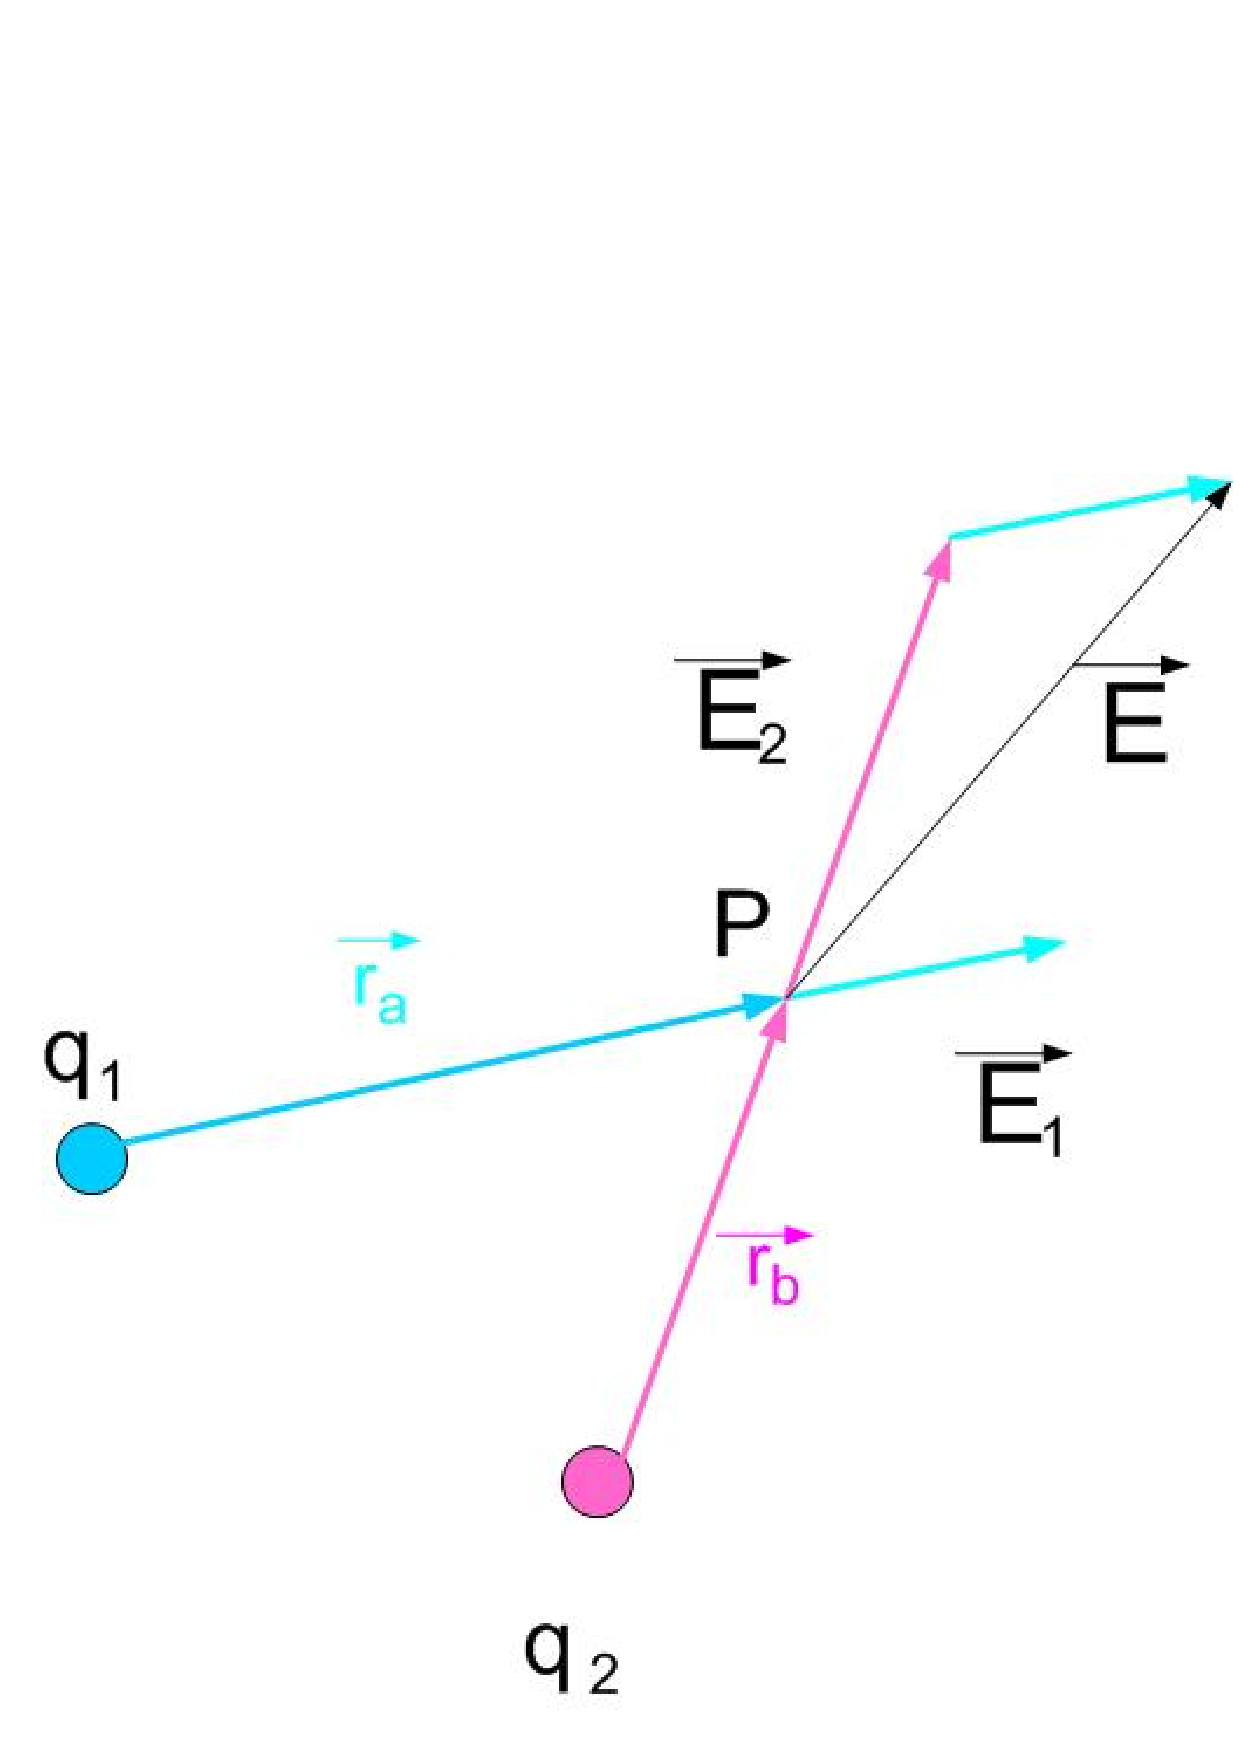
\includegraphics[scale=0.5]{../jpg/superposition.jpg}
\end{center}
\caption{Electric Field due to two charges.}
\label{superposition}
\end{figure}

The fields or charges $q_1$ and $q_2$ are:

\begin{eqnarray}
\vec{E_1}=\frac{q_1}{4 \pi \epsilon_{0} {r_a}^2} \hat{r_a} \label{field}\\
\vec{E_2}=\frac{q_1}{4 \pi \epsilon_{0} {r_b}^2} \hat{r_b}
\end{eqnarray}

Where $\hat{r_a}$ and $\hat{r_b}$ are unit vectors in the direction of $r_a$ and $r_b$. The total field due to both charges is


\begin{eqnarray}
\vec{E}=\vec{E_1} + \vec{E_2} 
\end{eqnarray}






\subsection{Electric Field in Rectangular Coordinates}


The general equation for the electric field is given as



\begin{eqnarray}
\vec{E}=\frac{q_1}{4 \pi \epsilon_{0} {r_a}^2} \hat{r_a} \label{genfield}
\end{eqnarray}

The electric field at a point $P(x,y,z)$ due to a charge $q_1$ positioned at a point $P_{q_1}(x_1, y_1, z_1 )$  in the rectangular coordinate system is shown in Figure \ref{singlecharge1}. The position vector of the point $P_{q_1}$  is 


\begin{figure}[htbp]
\begin{center}
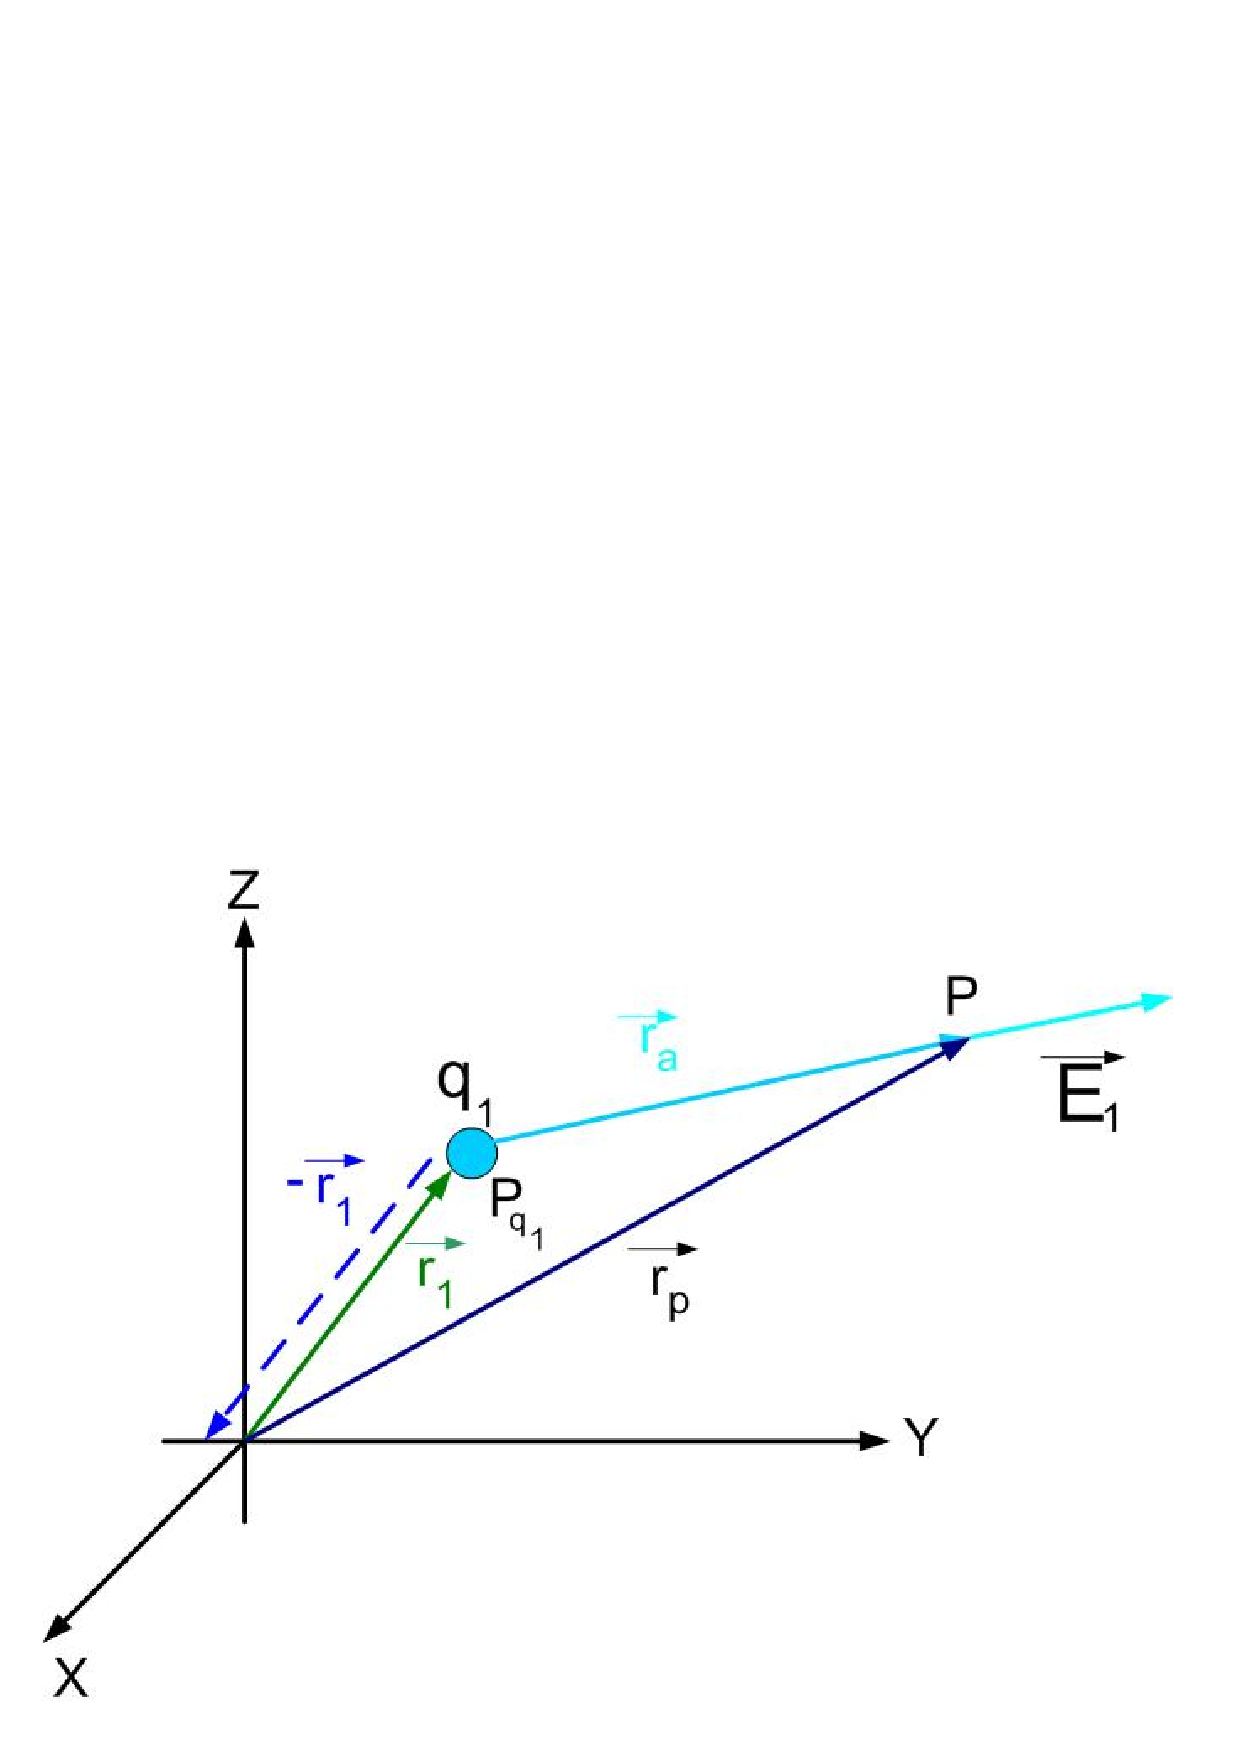
\includegraphics[scale=0.5]{../jpg/singlechargecartcoord.jpg}
\end{center}
\caption{Electric Field due to a unit charge in Rectangular coordinate system.}
\label{singlecharge1}
\end{figure}





\begin{eqnarray}
\vec{r_1}=x_1 \vec{x} + y_1 \vec{y} +z_1 \vec{z}
\end{eqnarray}

The position vector of point $P$ is equal to

\begin{eqnarray}
\vec{r_p}=x\vec{x} + y \vec{y} +z \vec{z}
\end{eqnarray}

The two vectors mark the beginning and the end of the distance vector $\vec{r_a}$  between points $P_{q_1}$ and $P$. The vector  $\vec{r_a}$ is the sum of vectors $-\vec{r_p}$ and $\vec{r_1}$



\begin{eqnarray}
\vec{r_a}=\vec{r_p} + (-\vec{r_1})
\end{eqnarray}

When we substitute position vectors $r_1$ and $r_p$:

\begin{eqnarray}
\vec{r_a}= (x - x_1) \vec{x} +(y - y_1) \vec{y} +(z - z_1) \vec{z}
\end{eqnarray}

Vector $\vec{r_a}$ has the magnitude of:


\begin{eqnarray}
|\vec{r_a}|= \sqrt{(x - x_1)^2 +(y - y_1)^2 +(z - z_1)^2}
\end{eqnarray}

Unit vector in the direction of vector $\vec{r_a}$ is:


\begin{eqnarray}
\hat{r_a}= \frac{\vec{r_a}}{|\vec{r_a}|} \\
\hat{r_a}=\frac{\vec{r_a}}{\sqrt{(x - x_1)^2 +(y - y_1)^2 +(z - z_1)^2}}
\end{eqnarray}



\begin{eqnarray}
\vec{E_1}=\frac{q_1}{4 \pi \epsilon_{0} {r_a}^2} \hat{r_a}
\end{eqnarray}

Where $r_a$ is the distance between the charge $q_1$ and the point $P$. Substituting expressions for $\hat{r_a}$, and $|\vec{r_a}|$ in equation \ref{genfield} we get

 



\begin{eqnarray}
\vec{E_1}=\frac{q_1}{4 \pi \epsilon_{0} {\sqrt{(x - x_1)^2 +(y - y_1)^2 +(z - z_1)^2}
}^3} \vec{r_a} \label{eqonecharge}
\end{eqnarray}

Substituting 


For two charges, as shown in Figure \ref{twocharges} equation \ref{eqonecharge} becomes

\begin{eqnarray}
\vec{E}= \frac{q_1}{4 \pi \epsilon_{0} {\sqrt{(x - x_1)^2 +(y - y_1)^2 +(z - z_1)^2}
}^3} \vec{r_a} + \nonumber \\ \frac{q_2}{4 \pi \epsilon_{0} {\sqrt{(x - x_2)^2 +(y - y_2)^2 +(z - z_2)^2}
}^3} \vec{r_b} 
\end{eqnarray}


\begin{figure}[htbp]
\begin{center}
\includegraphics[scale=0.5]{../jpg/twochargescartcoord.jpg}
\end{center}
\caption{Electric field due to two charges in  Rectangular coordinate system.}
\label{twocharges}
\end{figure}






\begin{example}
Find the point P where total electric field is zero inside of an equilateral triangle, if the three charges of magnitude 3\,nC, 3\,nC, and 3\,nC are placed in the corners of equilateral triangle of side 2\,m. Use the app below to confirm your result.
\begin{center}  
\geogebra{kupge9gc}{1200}{800}  
\end{center} 
\end{example}



\end{document} 

